\subsection{一致空间的拓扑}

命题 1 设 X 是赋有一致结构 U 的集合，对每个 \(x \in X\)，令 \(\mathfrak{B}(x)\) 为诸子集 \(\mathbf{V}(x)\)（\(\mathbf{X}(*)\) 的子集）组成的集，其中 V 取遍 U 的一致邻域集。则 X 上存在唯一的拓扑，使对每个 \(x \in X\)，\(\mathfrak{B}(x)\) 是 x 在该拓扑中的邻域滤子。

必须证明诸 \(\mathfrak{B}(x)\) 满足第一章 § 1 第 2 目的条件 \((\mathbf{V}_{\mathbf{I}})\)、\((\mathbf{V}_{\mathbf{II}})\)、\((\mathbf{V}_{\mathbf{III}})\) 与 \((\mathbf{V}_{\mathbf{IV}})\)。对前三个条件而言，这可由 \(\mathcal{U}\) 的诸一致邻域满足 \((\mathbf{F}_{\mathbf{I}})\)、\((\mathbf{F}_{\mathbf{II}})\) 与 \((\mathbf{U}_{\mathbf{I}})\) 立即得出。至于 \((\mathbf{V}_{\mathbf{IV}})\)，设 \(\mathbf{V}\) 是 \(\mathcal{U}\) 的一个一致邻域，\(\mathbf{W}\) 是 \(\mathcal{U}\) 的使 \(\hat{\mathbf{W}} \subset \mathbf{V}\) 的一致邻域；则当 \((x, y) \in \mathbf{W}\) 且 \((y, z) \in \mathbf{W}\) 时有 \((x, z) \in \mathbf{V}\)，从而 \(\mathbf{W}(y) \subset \mathbf{V}(x)\) 对一切 \(y \in \mathbf{W}(x)\) 成立，因此 \(\mathbf{V}(x) \in \mathfrak{B}(y)\) 对一切 \(y \in \mathbf{W}(x)\) 成立。证毕。

定义 3 命题 1 中所定义的拓扑称为一致结构 U 诱导的拓扑。

例。* 1）加法一致结构在实数集上诱导的拓扑是实直线的拓扑（第一章 § 1 第 2 目）；类似地，加法一致结构在有理数集上诱导的拓扑是有理直线的拓扑。*

\begin{enumerate}
\def\labelenumi{\arabic{enumi})}
\setcounter{enumi}{1}
\tightlist
\item
  在任何集合 X 上，离散一致结构（第 1 目例 2）诱导的拓扑都是离散拓扑。
\end{enumerate}

今后当我们谈到一致空间 X 的拓扑时，除非另有明确说明，总是指该空间的一致结构所诱导的拓扑。在集合 X 上赋以这个拓扑所得到的拓扑空间，有时称为所说一致空间的底拓扑空间。例如，当我们说一个一致空间是豪斯多夫的、或紧的、或局部紧的等等时，我们是指其底拓扑空间具有该性质。

若 X 与 \(X'\) 是两个一致空间，则 X 的一致结构到 \(X'\) 的一致结构上的任一同构 f 也是 X 到 \(X'\) 上的同胚；我们称 f 是一致空间 X 到一致空间 \(X'\) 上的同构。应当注意，X 到 \(X'\) 上的同胚未必是 X 的一致结构到 \(X'\) 的一致结构上的同构。

\pandocbounded{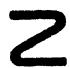
\includegraphics[keepaspectratio]{images/part001_037a61a5.jpg}}

换句话说，同一集合 X 上不同的一致结构可以诱导同一拓扑。* 例如，在 {]}0, +∞{[} 上，加法一致结构与乘法一致结构（它们是不同的：第三章 § 6 习题 17）诱导同一拓扑。*

另一个例子见 § 2 第 2 目注 1。

命题 2 设 X 是一致空间。对 X 的每个对称一致邻域 V 与 X × X 的每个子集 M，VMV 是 M 在积空间 X × X 中的邻域，且 M 在此空间中的闭包由下列公式给出

\[
\overline {{\mathbf {M}}} = \bigcap_ {\mathbf {V} \in \mathfrak {S}} \mathbf {V M V}\tag{I}
\]

其中 \(\mathfrak{S}\) 表示 \(\mathbf{X}\) 的对称一致邻域组成的集。

设 V 是 X 的一个对称一致邻域。关系 \((x, y) \in \text{VMV}\) 表示存在 M 的元素 \((p, q)\) 使 \((x, p) \in V\) 且 \((q, y) \in V\)：换句话说（因 V 对称），\(x \in V(p)\) 且 \(y \in V(q)\)，即 \((x, y) \in V(p) \times V(q)\)。由于 \(V(p) \times X(q)\) 是 \((p, q)\) 在 \(X \times X\) 中的邻域，命题的第一部分得证。关系 \((x, p) \in V\) 与 \((y, q) \in V\) 也可写成 \(p \in V(x)\)、\(q \in V(y)\) 或 \((p, q) \in V(x) \times V(y)\)。当 V 取遍 S 时，诸集合 \(V(x) \times V(y)\) 构成 \((x, y)\) 在 \(X \times X\) 中的基本邻域系；因为若 U 与 \(U'\) 是任意两个一致邻域，总存在对称一致邻域 \(V \subset U \cap U'\)，使 \(V(x) \times V(y) \subset U(x) \times U'(y)\)。因此，\(V(x) \times V(y)\) 对每个 \(V \in S\) 都与 M 相交，当且仅当 \((x, y) \in \overline{\mathbf{M}}\)，由此即得公式 (1)。

推论 1 若 A 是 X 的任一子集，V 是 X 的任一对称一致邻域，则 V(A) 是 A 在 X 中的邻域，且

\[
\overline {{{\mathbf {A}}}} = \bigcap_ {\mathbf {v} \in \mathfrak {S}} \mathbf {V} (\mathbf {A}) = \bigcap_ {\mathbf {v} \in \mathfrak {U}} \mathbf {V} (\mathbf {A})\tag{2}
\]

其中 \(\mathfrak{U}\) 表示 \(\mathbf{X}\) 中所有一致邻域组成的集。

若 \(\mathbf{M} = \mathbf{A} \times \mathbf{A}\)，则 \(\mathrm{VMV} = \mathrm{V}(\mathbf{A}) \times \mathrm{V}(\mathbf{A})\) 对任何 \(\mathbf{V} \in \mathfrak{S}\) 成立；因为关系“存在 \(p \in \mathbf{A}\) 使 \((x, p) \in \mathbf{V}"\)按定义等价于 \(x \in \mathbf{V}(\mathbf{A})\)。推论由第一章 § 4 第 2 目命题 5 与第 3 目命题 7 立即得出。

V(A) 称为 A 的 V-邻域。

若 V 是在 X × X 中开的一致邻域，则对每个 x ∈ X，V(x) 在 X 中开（第一章 § 4 第 2 目命题 4 的推论），因此 V(A)——它是 x 取遍 A 时诸 V(x) 的并——在 X 中开。另一方面，若 V 是 X × X 中的闭一致邻域，则对 X 的每个子集 A，V(A) 未必在 X 中闭（习题 3）。

\pandocbounded{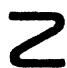
\includegraphics[keepaspectratio]{images/part001_f8cd4ad5.jpg}}

还应指出，当 V 取遍 X 的一致邻域集时，诸集合 V(A) 未必构成 A 在 X 中的基本邻域系（习题 2）。

推论 2 X 的一致邻域在 X × X 中的内部（相应地，闭包）构成 X 的一个一致邻域基本系。

若 V 是 X 的任一一致邻域，则存在对称一致邻域 W 使 \(W \subset V\)；由于 W 是 W 的邻域（命题 2），V 在 \(X \times X\) 中的内部含 W，从而是一个一致邻域。此外，由命题 2 有 \(W \subset W \subset W \subset V\)，因此 V 含某个一致邻域的闭包。

推论 3 每个一致空间都满足公理（O \(_{III}\)）。

若 \(x\) 是 \(X\) 的任一点且 \(V\) 取遍 \(X\) 的在 \(X \times X\) 中闭的一致邻域，则由推论 2，诸集合 \(V(x)\) 构成 \(x\) 在 \(X\) 中的基本邻域系，并且它们在 \(X\) 中闭（第一章 § 4 第 2 目命题 4 的推论）。

命题 3 一致空间 X 是分离的，当且仅当其一致结构的所有一致邻域之交是对角线 \(\Delta\)（即 \(X \times X\) 的对角线）。每个分离的一致空间都是正则的。

后一断言由命题 2 的推论 3 立即得出。我们已看到，闭的一致邻域构成一个一致邻域基本系（命题 2 推论 2）；若其交是 \(\Delta\)，则 \(\Delta\) 在 \(X \times X\) 中闭，从而 \(X\) 是分离的（第一章 § 8 第 1 目命题 1）。反之，若 \(X\) 分离，则对每个点 \((x, y) \notin \Delta\)，存在 \(V\)（\(X\) 的一致邻域）使 \(y \notin V(x)\)，或等价地 \((x, y) \notin V\)；于是 \(\Delta\) 是所有一致邻域之交。

若一致空间 X 分离，我们就说 X 的一致结构是分离的。若 B 是该结构的一个一致邻域基本系，则 X 分离当且仅当 B 中所有集合之交是 \(\Delta\)。

